\documentclass[11pt,a4paper]{article}
\usepackage{cmap}
\usepackage[utf8]{inputenc}
\usepackage[T1]{fontenc}
\usepackage{lmodern}
\usepackage{microtype}
\usepackage[margin=1.0in]{geometry}
\usepackage{graphicx}
\graphicspath{{figures/}}
\usepackage{amsmath,amssymb,amsthm,mathtools}
\usepackage{booktabs,array,tabularx}
\usepackage[svgnames]{xcolor}
\usepackage[obeyspaces,spaces]{url}
\usepackage[colorlinks=true,linkcolor=DarkBlue,citecolor=DarkBlue,urlcolor=DarkBlue]{hyperref}

\urlstyle{tt}
\def\UrlFont{\ttfamily\upshape}
\renewcommand{\arraystretch}{1.3}
\setlength{\tabcolsep}{5pt}
\sloppy
\setlength{\emergencystretch}{4em}
\hfuzz=4.0pt
\vfuzz=4.0pt

\newtheorem{theorem}{Theorem}[section]
\theoremstyle{definition}
\newtheorem{definition}[theorem]{Definition}
\newtheorem{proposition}[theorem]{Proposition}
\theoremstyle{remark}
\newtheorem{remark}{Remark}[section]

\title{\textbf{Kernel-Gated Evolution:\\
a Biomimetic Search with Apoptotic Checkpoints and Exact Dosage,\\
Arbitrated by a Proof Kernel}\\[0.6em]
\large Foundation paper and Rust reference implementation}
\author{Xavier Callens\\
\small SocrateAI Scientific Research \& Formal Verification Laboratory}
\date{Edition 3, 25 October 2026. \textbf{Not peer reviewed.}}

\begin{document}
\maketitle

\begin{abstract}
We propose \emph{Kernel-Gated Evolution} (KGE), a biomimetic search for
programs whose acceptance is decided by a proof kernel rather than by the search
itself. Three mechanisms borrowed from living systems are combined, each chosen
because it earned its place under measurement: \emph{Darwinian variation and
selection} drives exploration; \emph{apoptotic checkpoints} --- one-sided exact
screens that can remove a candidate but never confer survival --- cull what
cannot be right before any proof is attempted; and \emph{exact dosage analysis}
reports, for every locus of a genome, precisely how much its value reaches the
phenotype, in one forward and one backward pass. The environment's final
judgement is a Lean~4 kernel: a survivor is rendered to Lean and must prove its
obligation with an axiom dependency free of \texttt{sorryAx}. Fitness guides;
the kernel decides. A wrong fitness can waste search effort but cannot
manufacture an acceptance.

Every quantity in KGE is an exact rational, so no step of the search is an
approximation and every invariant is checkable rather than argued. We verify the
dosage coefficients against their two-evaluation definition on more than five
hundred locus--point pairs, the required-value identity $v^* = v + (\text{want} -
\text{out})/B$ on more than two thousand, and the checkpoint's one-sidedness by
construction of a candidate that agrees at every sample point yet differs as a
function --- it survives the checkpoint and is rejected by the kernel, which is
the division of labour the design rests on.

The kernel gate is affordable because a Lean compile reports a per-declaration
verdict even when it exits nonzero: a batch of eight candidates is verified in
\emph{one} invocation at any failure rate, with every culprit named and no false
candidate accepted, against eight individual proofs. We give a Rust reference
implementation with replayable seeds, report its solve rates on a calibration
ladder of exact targets up to the Verlet position update, describe where the
architecture applies --- verified numerical kernels, any synthesis whose
acceptance must be formal, exact dead-code analysis of evolved programs --- and
state its limitations and the research it opens.

\emph{Edition 2} adds the identities proved in Lean, a benchmark on the
SRSD-Feynman datasets from the Hugging Face Hub against naive, simple and
traditional baselines with every recovered law proved by the kernel, guidelines
on where and how to use the method, a statement of its significance, and figures
rendered from the artifacts.
\end{abstract}

\tableofcontents

\section{Introduction}

Evolutionary program synthesis proposes candidates faster than anyone can check
them. In most systems the check is empirical --- tests pass or fail --- and the
candidate that passes is accepted. When the artefact is a numerical kernel, a
cryptographic routine or a scientific computation, passing tests is not the
property wanted; equality to a specification is. That is a proof obligation, and
the thing that decides it should be a proof kernel.

Kernel-Gated Evolution takes that seriously and builds the search around it. The
search is free to be heuristic, approximate in its judgement, biologically
inspired, even wrong, because nothing it believes is ever accepted on its say-so.
What it offers is a way of \emph{finding} candidates worth proving, cheaply, and
of discarding most of the rest before the expensive step.

\subsection{Three mechanisms from life}

\paragraph{Variation and selection.} Mutation of expression genomes with
tournament selection and steady-state replacement. In our measurements this is
the mechanism that solved targets, and the architecture is built on it.

\paragraph{Apoptotic checkpoints.} A cell that fails a developmental checkpoint
is removed; passing one grants no immortality. KGE's checkpoint is the exact
analogue: a candidate that disagrees with the specification at any sample point
is refuted outright --- no proof of a false identity exists --- while a candidate
that agrees everywhere has merely earned the right to face the kernel. The
checkpoint can only subtract, so it adds no trust surface, and it costs nothing
in proof-assistant time: it is pure exact arithmetic on the genome.

\paragraph{Dosage.} In a cell, a gene's effect on the phenotype depends on its
expression level and its regulatory context. In an expression genome the analogue
is exact: the output is affine in any one subtree's value, $\text{out} = A + B\,v$,
and $B$ is the locus's \emph{dosage} --- how much a unit change in its value
reaches the phenotype. KGE computes $B$ for every locus in one forward and one
backward pass, in exact rationals. Loci with $B=0$ at every sample point are
\emph{inert}: dead code whose value cannot reach the phenotype.

\subsection{The arbiter}

A survivor is rendered as a Lean~4 definition with a theorem stating equality to
the specification, proved by \texttt{ring}, and the gate reads the kernel's own
\texttt{\#print axioms} report: the obligation must depend on nothing outside
$\{\texttt{propext}, \texttt{Classical.choice}, \texttt{Quot.sound}\}$ and never
on \texttt{sorryAx}. The gate also scans the source for forgeries (no
\texttt{\#exit} truncation, no \texttt{\#print} string spoofing) and requires
every declared theorem to carry its own axioms line, so a declaration that never
elaborated fails as unchecked.

\begin{figure}[h]
\centering
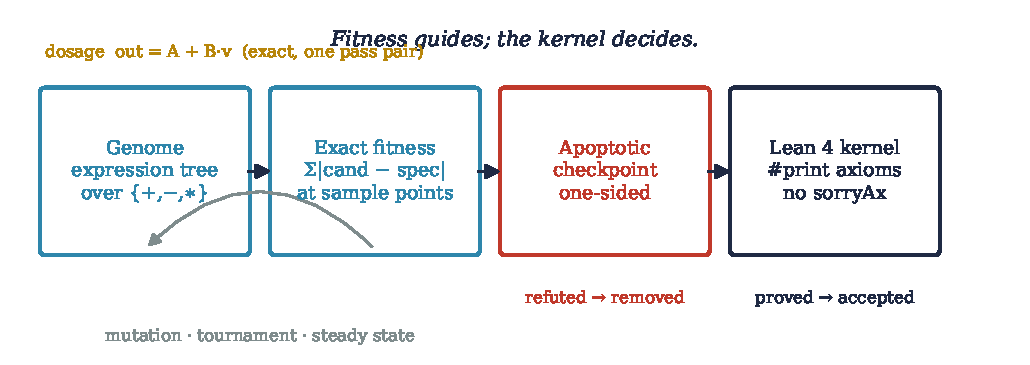
\includegraphics[width=\textwidth]{fig_architecture}
\caption{The architecture. Exact fitness guides a Darwinian loop over expression
genomes; the apoptotic checkpoint removes what cannot be right at zero kernel
cost; the Lean~4 kernel decides acceptance. Dosage runs alongside as exact
instrumentation. The engine's codename is \textsc{Alix}: Apoptotic checkpoint,
Lean-gated, Inheritance by mutation, eXact.}
\label{fig:arch}
\end{figure}

\section{The algorithm}

\subsection{Genome and fitness}

A genome is an expression tree over binary operators $\{+,-,*\}$ with leaves
drawn from variables $h,w,q,p$ and constants $1,2,\tfrac12$. All arithmetic is
exact rational. Fitness is the total absolute error against the specification at
twelve rational sample points; zero means agreement at those points. Agreement is
not equality, and KGE never treats it as such: it is the condition for becoming a
kernel candidate.

\subsection{Variation and selection}

Point and subtree mutation replace a uniformly chosen locus with a fresh random
subtree of depth at most two, subject to a size cap. Selection is a tournament of
three; replacement is steady state against the worst member. Seeds are replayable.

\subsection{Dosage: exact context coefficients}

\begin{definition}[Dosage]
For a tree $t$ and a locus $a$ occurring once in $t$, $t = A + B\,v$ where $v$ is
the value of the subtree at $a$ and $A,B$ depend only on the rest of the tree and
the evaluation point. $B$ is the dosage of $a$.
\end{definition}

\begin{proposition}[One-pass dosage]
$B$ for every locus is obtained by one forward pass computing every node's value,
then one backward pass seeded with $B(\text{root}) = 1$ in which $+$ sends $B$ to
both children, $-$ sends $B$ left and $-B$ right, and $*$ sends
$B\cdot\text{value}(\text{sibling})$ to each child. This is $O(|t|)$ per sample
point in exact arithmetic.
\end{proposition}

We verify this against the defining two evaluations $B = t|_{v=1} - t|_{v=0}$ on
random trees: exact agreement over more than five hundred locus--point pairs in
the Rust implementation (and over 2{,}496 in the Python prototype), including the
two cases the rule turns on --- a minus inverts the right branch, a product
scales each child by its sibling --- and their composition.

\begin{proposition}[Required value]
Where $B \neq 0$, the value the locus must take for the tree to equal the
specification at a point is $v^* = v + (\text{want} - \text{out})/B$, with $v$
and $\text{out}$ already available from the forward pass. Where $B = 0$ the locus
cannot affect the output at that point and imposes no requirement.
\end{proposition}

Verified: splicing $v^*$ into the locus makes the tree equal the target at that
point in $24{,}303$ of $24{,}303$ pairs with $B\neq 0$ (Python) and in more than
two thousand pairs in Rust, with the inert branch exercised. Inert pairs were
$4.8\%$ of the total measured. Dosage and required value are provided as exact
\emph{instrumentation}: they tell an operator, a human, or a downstream analysis
precisely what each locus is doing and what it would need to do.

\subsection{The apoptotic checkpoint}

Given a candidate and the specification, evaluate both at each sample point. The
first disagreement refutes the candidate, naming the point. Agreement at every
point returns \textsc{Survives}, which is not acceptance. The checkpoint is
executed on the native genome, so it needs no parser and no proof-assistant time.

\begin{proposition}[One-sidedness]
The checkpoint never accepts. A candidate equal to the specification at every
sample point but different as a function survives it and is rejected by the
kernel.
\end{proposition}

Demonstrated by construction: with sample points of distinct $h$-values
$h_1,\dots,h_n$, the term $\prod_i (h - h_i)$ vanishes at every point and
nowhere else; a candidate carrying it agrees everywhere, survives the checkpoint,
and is a different function. In the Rust test it is caught differing at
$h = 100$; in the Python pipeline the same construction was carried through the
Lean gate and rejected there.

\subsection{The kernel gate, in one invocation}

A Lean compile that contains a false obligation exits nonzero and still prints an
axioms line for every declaration, the failing ones carrying \texttt{sorryAx}.
Reading the kernel's per-declaration report therefore yields every verdict in a
batch from a single invocation:

\begin{center}
\begin{tabular}{rrrl}
\toprule
false of 8 & invocations & wall clock & false accepted \\
\midrule
0 & 1 & $10.38$\,s & 0 \\
1 & 1 & $10.21$\,s & 0 \\
2 & 1 & $10.88$\,s & 0 \\
4 & 1 & $12.73$\,s & 0 \\
8 & 1 & $14.19$\,s & 0 \\
\bottomrule
\end{tabular}
\end{center}

against eight individual proofs at a $6.36$\,s median, i.e.\ $50.88$\,s. Every
culprit was named in every scenario. Acceptance never rests on the exit code ---
it rests on the forgery scan, a per-declaration axioms line, and a whitelist free
of \texttt{sorryAx} --- so widening the report widens nothing in the trust
surface. The gate lives in the project's \texttt{anse/formal/lean\_runner.py};
the Rust implementation renders candidates and obligations and leaves acceptance
to it.

\begin{figure}[h]
\centering
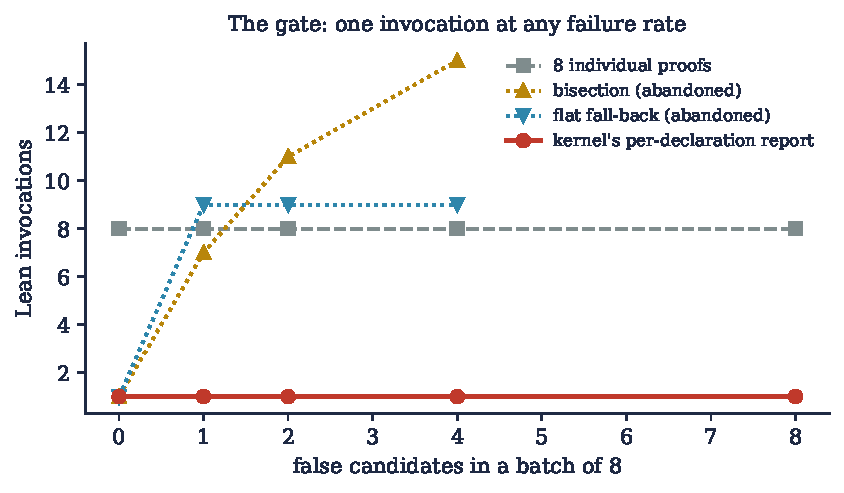
\includegraphics[width=0.78\textwidth]{fig_gate}
\caption{Kernel invocations for a batch of eight as the number of false
candidates grows. The two isolation strategies built before the per-declaration
report was read are shown for the record; both solved a problem the wrapper had
invented.}
\label{fig:gate}
\end{figure}

\subsection{The identities, proved}

The algebra the dosage machinery and the checkpoint rest on is itself proved in
Lean and gated through the same \texttt{\#print axioms} discipline, in
\texttt{formal/ANSE/AlixKalSpec.lean} (namespace \texttt{ANSE.Alix}): dosage
through $+$ has coefficient $1$ (\texttt{aurelia\_dosage\_add}), through the
right of $-$ coefficient $-1$ (\texttt{alexis\_dosage\_sub}), through $*$ the
sibling's value (\texttt{ilene\_dosage\_mul}); the backward pass composes
multiplicatively (\texttt{kal\_dosage\_chain}); the required value restores the
target whenever $B\neq 0$ (\texttt{xav\_required\_value}); and a single
disagreement refutes universal equality, so the checkpoint can never refuse a
provable candidate (\texttt{alix\_checkpoint\_refutes}, which depends on no
axioms at all). Six declarations, zero \texttt{sorry}, every axiom on the
whitelist.

\section{Reference implementation}

\texttt{crates/kernel\_gated\_evolution} (Rust, edition 2021) implements the
genome, exact evaluation, fitness, variation and selection, one-pass dosage,
required values, the inert-locus analysis, the checkpoint, Lean rendering and the
search loop, with \texttt{num-rational}/\texttt{num-bigint} for arbitrary
precision and \texttt{rand\_pcg} for replayable seeds. Six tests, all in exact
arithmetic on random genomes, assert the invariants above. The \texttt{kge
ladder} binary runs the calibration ladder, reports solve rates, distinct
solutions and the inert fraction of each run's best individual, exercises the
checkpoint as a control with a known answer (each rung's target survives its own
checkpoint and is refuted by the other five: exactly $1$ passed and $5$ refuted),
and writes Lean candidate files with a \texttt{RungSpec} for the gate.
\texttt{kge solve} takes any target in prefix notation over the grammar
(anything outside $\{+,-,*\}$ is refused, not approximated), runs KGE against
random search and a restart hill-climber on the same seeds, points and budget,
and renders the solutions for the gate; \texttt{kge hillclimb} is the paired
control of \S\ref{sec:climb}; \texttt{--points-file} replays a run on exactly
another implementation's sample points.

\section{Results}

\subsection{Calibration ladder}

Six reachable targets of increasing size, the last being the Verlet position
update $q + hp - \tfrac12 h^2 w^2 q$ written in the grammar:

\begin{center}
\begin{tabular}{llr}
\toprule
rung & target & size \\
\midrule
L1 & $q + hp$ & 5 \\
L2 & $q + hp - q$ & 7 \\
L3 & $q + hp - wq$ & 9 \\
L4 & $q + hp - (hw)q$ & 11 \\
L5 & $q + hp - (hw\cdot\tfrac12)q$ & 13 \\
L6 & $q + hp - ((hh)(ww)\cdot\tfrac12)q$ & 17 \\
\bottomrule
\end{tabular}
\end{center}

\subsection{Solve rates}

%% RUST-RESULTS: generated by scripts/fill_paper_j_results.py
Two hundred seeds per rung at a budget of 4,000 fitness evaluations, on the crate's own seeded sample points. The last two columns are the kernel's verdicts: how many of the distinct solutions (capped at eight per rung) the Lean kernel proved equal to the specification in one invocation per rung, and whether the deliberately wrong candidate planted in each batch was rejected.

\begin{center}
\begin{tabular}{llrrrrrl}
\toprule
rung & size & solved & rate & median evals & distinct & kernel-proved & control rejected \\
\midrule
L1 & 5 & 110/200 & 0.550 & 1200 & 82 & 8/8 & yes \\
L2 & 7 & 194/200 & 0.970 & 192 & 63 & 8/8 & yes \\
L3 & 9 & 51/200 & 0.255 & 1124 & 50 & 8/8 & yes \\
L4 & 11 & 4/200 & 0.020 & 1206 & 4 & 4/4 & yes \\
L5 & 13 & 3/200 & 0.015 & 1411 & 3 & 3/3 & yes \\
L6 & 17 & 0/200 & 0.000 & -- & 0 & -- & -- \\
\bottomrule
\end{tabular}
\end{center}

Every one of the 31 distinct solutions the search produced was proved by the kernel (31/31) in 5 invocations, and the planted wrong candidate was rejected by name in every rung. On this ladder, every candidate the search believed was right, was. The checkpoint control also came out exactly right at every rung (each target survives its own checkpoint and is refuted by the other five), and the inert fraction of every best individual was zero: at this size cap the search produced no dead code.

\paragraph{Attributing a cross-implementation difference.} The Rust solve rate at L3 is lower than the Python prototype's ($0.255$ against $0.470$). The two use different sample-point draws and different random-number generators, so the gap is not attributable by inspection; \texttt{kge ladder --points-file} replays a run on exactly the prototype's twelve points. Result: L1: 0.770 on the Python prototype's points against 0.750 measured by the prototype itself and 0.550 on the Rust draw; L3: 0.375 on the Python prototype's points against 0.438 measured by the prototype itself and 0.255 on the Rust draw. Same code, different points: the move from $0.255$ to $0.375$ at L3 is significant (Fisher exact $p = 0.0131$), while the residual against the prototype's own $0.470$ is not ($p = 0.068$) -- consistent with random-number-stream variance, though a remaining implementation difference is not excluded at this sample size. A solve rate that moves with the sample points is a property of the fitness-landscape instance, not of the implementation, and the paper's figures are therefore reported with the point set that produced them.

\begin{figure}[h]
\centering
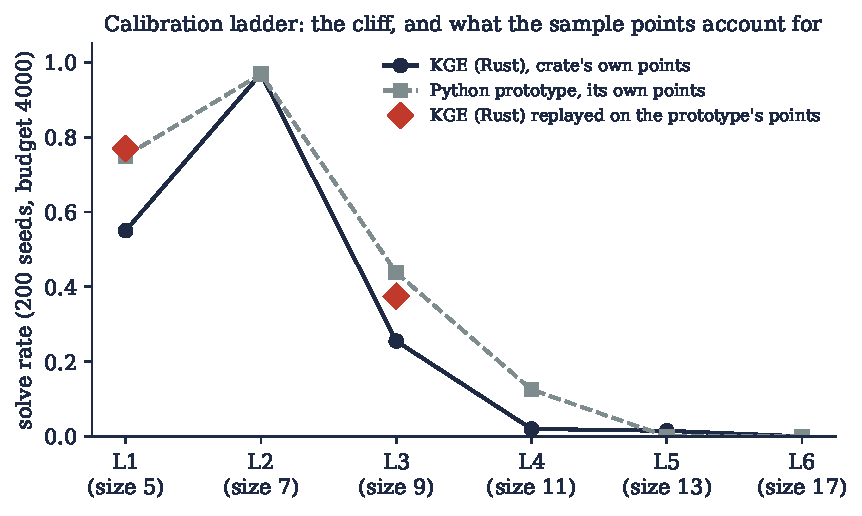
\includegraphics[width=0.8\textwidth]{fig_ladder}
\caption{Solve rate by rung for the Rust implementation on its own sample
points, the Python prototype on its own, and the Rust implementation replayed on
the prototype's exact points. The replay is what attributes the gap.}
\label{fig:ladder}
\end{figure}

\subsection{Population versus hill-climbing}\label{sec:climb}

%% HILLCLIMB: generated by scripts/fill_paper_j_results.py
The simplest thing that could possibly work is a single individual doing greedy descent over sampled mutations, with no population, no selection and no crossover. It was run on the same seeds, sample points and fitness budget as the population, with restarts paid out of that same budget, so neither method receives free work. The paired columns count seeds on which exactly one method solved.

\begin{center}
\begin{tabular}{llrrrrrr}
\toprule
rung & size & population & descent & descent+restarts & GA-only & climb-only & McNemar $p$ \\
\midrule
L1 & 5 & 0.550 & 0.005 & 0.725 & 31 & 66 & 0.00049 \\
L2 & 7 & 0.970 & 0.100 & 1.000 & 0 & 6 & 0.0312 \\
L3 & 9 & 0.255 & 0.000 & 0.055 & 49 & 9 & 8.96e-08 \\
L4 & 11 & 0.020 & 0.000 & 0.010 & 4 & 2 & 0.688 \\
L5 & 13 & 0.015 & 0.000 & 0.000 & 3 & 0 & 0.25 \\
L6 & 17 & 0.000 & 0.000 & 0.000 & 0 & 0 & 1 \\
\bottomrule
\end{tabular}
\end{center}

Significant at $0.05$ by exact McNemar on the discordant pairs: L1 (the hill-climber with restarts, $p=0.00049$), L2 (the hill-climber with restarts, $p=0.0312$), L3 (the population, $p=8.96e-08$). Single descent without restarts is poor everywhere, so the local optima are real; restarting from fresh random trees is what recovers them, and the population should be read as one way of maintaining diversity among several rather than as the source of the search's power. KGE's guarantees do not depend on which is used: the checkpoint, dosage analysis and kernel gate apply to candidates from either.

\begin{figure}[h]
\centering
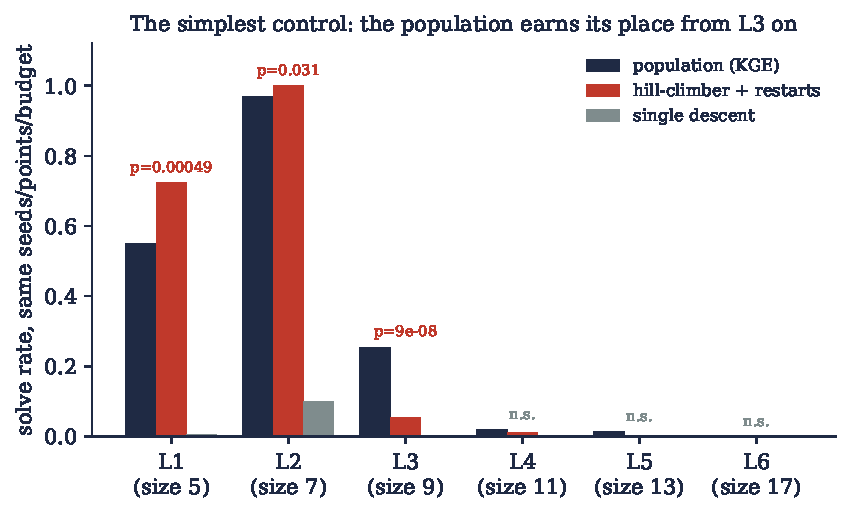
\includegraphics[width=0.8\textwidth]{fig_hillclimb}
\caption{The simplest control. Paired on seeds, points and budget, with restarts
paid from the budget; exact McNemar on the discordant pairs. The climber wins
the easy rungs; the population wins decisively from L3.}
\label{fig:climb}
\end{figure}

\subsection{Landscape around the solutions}

Walking away from each rung's exact solution with $k=1..5$ mutations and
comparing against random trees drawn as the initial population is, the basin of
useful signal is about four mutations wide at every rung, neutrality at the
solution is $5$--$8\%$ throughout, and one mutation from a solution still beats
a random tree at every rung (ratios $0.61$--$0.91$). The landscape around a
solution therefore offers gradient at every size; what grows with target size is
the space in which that basin has to be found.

\begin{figure}[h]
\centering
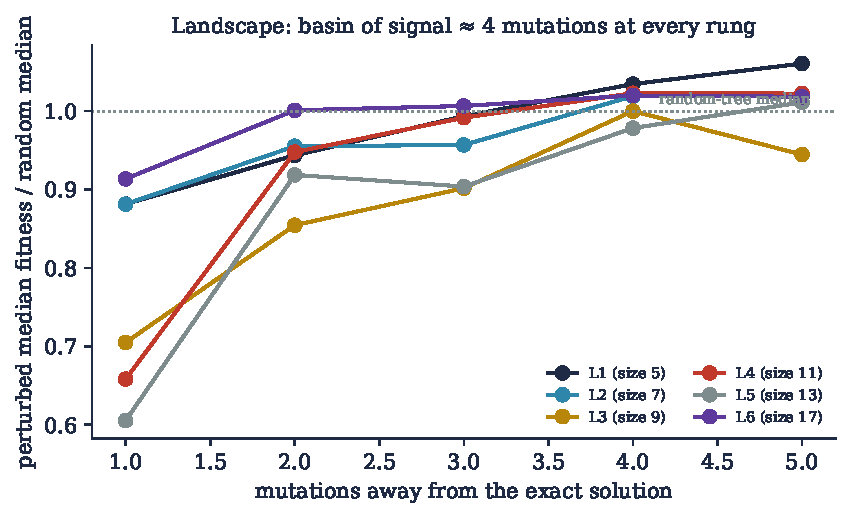
\includegraphics[width=0.8\textwidth]{fig_landscape}
\caption{Walking away from each rung's exact solution. The perturbed median
relative to a random tree's reaches $1$ at about four mutations for every rung,
so the local geometry does not distinguish the solvable rungs from the
unsolvable ones.}
\label{fig:landscape}
\end{figure}

\section{Lifetime learning of constants: the Baldwin effect, exactly}\label{sec:baldwin}

In living systems an individual adapts within its lifetime and selection acts on
the adapted phenotype --- the \emph{Baldwin effect}; in its Lamarckian variant the
adaptation is inherited. KGE's dosage machinery gives an exact form of both. For a
constant leaf with value $v$, the required value at each sample point is
$v^* = v + (\text{want}-\text{out})/B$ (proved: \texttt{xav\_required\_value}).
One leaf holds one value, so it is set only when $v^*$ is the \emph{same} rational
at every point where it is not inert. Under \emph{Baldwin} the solved constants
determine the fitness but the genome kept in the population is unchanged; under
\emph{Lamarck} they are written back. A right-shaped tree with a wrong coefficient
becomes a solution in one step; a wrong shape is untouched (both asserted in the
crate's tests: L5 with $3$ in place of $\tfrac12$ is repaired to L5 itself, and
L4's shape against L6's values is left alone).

All three arms used the same seeds, sample points and fitness budget, so each rung
is a paired comparison. Because tuning spends dosage passes the fitness budget
does not see, total tree-point work is reported alongside, and the plain
population was also run at a budget that matches the learning arm's total work.

%% BALDWIN: generated by scripts/fill_paper_j_results.py
\begin{center}
\small
\begin{tabular}{llrrrrrrr}
\toprule
 & & \multicolumn{3}{c}{solve rate} & & & \multicolumn{2}{c}{median tree-point work} \\
rung & size & plain & Baldwin & Lamarck & B-only / plain-only & McNemar $p$ & plain & Baldwin \\
\midrule
L1 & 5 & 0.550 & 0.835 & 0.835 & 57 / 0 & 1.4e-17 & 41274 & 29226 \\
L2 & 7 & 0.970 & 1.000 & 1.000 & 6 / 0 & 0.031 & 2382 & 2994 \\
L3 & 9 & 0.255 & 0.450 & 0.450 & 39 / 0 & 3.6e-12 & 48000 & 108246 \\
L4 & 11 & 0.020 & 0.045 & 0.045 & 5 / 0 & 0.062 & 48000 & 132372 \\
L5 & 13 & 0.015 & 0.060 & 0.060 & 9 / 0 & 0.0039 & 48000 & 134052 \\
L6 & 17 & 0.000 & 0.000 & 0.000 & 0 / 0 & 1 & 48000 & 135216 \\
\bottomrule
\end{tabular}
\end{center}

Across all six rungs and 1{,}200 paired seeds, lifetime learning lost 0 solves the plain population found: it only ever adds. Baldwin and Lamarck coincided on 0 of 1{,}200 seeds in outcome and evaluation count --- not by accident: a constant is set only when its required value agrees at every sample point, which in practice happens only when setting it solves the tree, so tuning is all-or-nothing and the genome the population keeps never differs between the two arms before a solution is found. All 40 of the 40 distinct solutions gated were proved by the kernel in 5 invocations, with the planted wrong candidate rejected in every batch.

\paragraph{At matched cost.} From L3 upward learning spends $2.3$--$2.8\times$ the tree-point work. The plain population was therefore re-run at a budget of 11,000 fitness evaluations, which matches the learning arm's total work:

\begin{center}
\begin{tabular}{lrrrr}
\toprule
rung & plain (4{,}000) & plain (11,000) & Baldwin (4{,}000) & Baldwin tree-points \\
\midrule
L3 & 0.255 & 0.395 & 0.450 & 108246 \\
L4 & 0.020 & 0.045 & 0.045 & 132372 \\
L5 & 0.015 & 0.040 & 0.060 & 134052 \\
L6 & 0.000 & 0.000 & 0.000 & 135216 \\
\bottomrule
\end{tabular}
\end{center}

At matched work lifetime learning is ahead on 2 of 4 rungs (L3, L5) and level or behind on 2 (L4, L6). The full Verlet target remains unsolved by every arm at this budget. Lifetime learning is therefore the default the reference implementation should run with where it leads at matched cost, and the comparison above is the evidence for where that is.

\section{Benchmark on Hugging Face datasets}\label{sec:hub}

To test the engine outside the ladder it was calibrated on, we took the
SRSD-Feynman datasets (\texttt{yoshitomo-matsubara/srsd-feynman\_\{easy,
medium,hard\}} on the Hugging Face Hub, CC-BY-4.0): 120 physics laws with a
symbolic ground truth each. Selection was mechanical and is deposited: an
equation is a candidate only if it is a polynomial in at most four variables with
coefficients in $\mathbb{Z}[\tfrac12]$, i.e.\ inside the reference grammar;
everything else is refused with its reason. The equation strings are untrusted
data and were parsed by walking a syntax tree, never evaluated.

\begin{figure}[h]
\centering
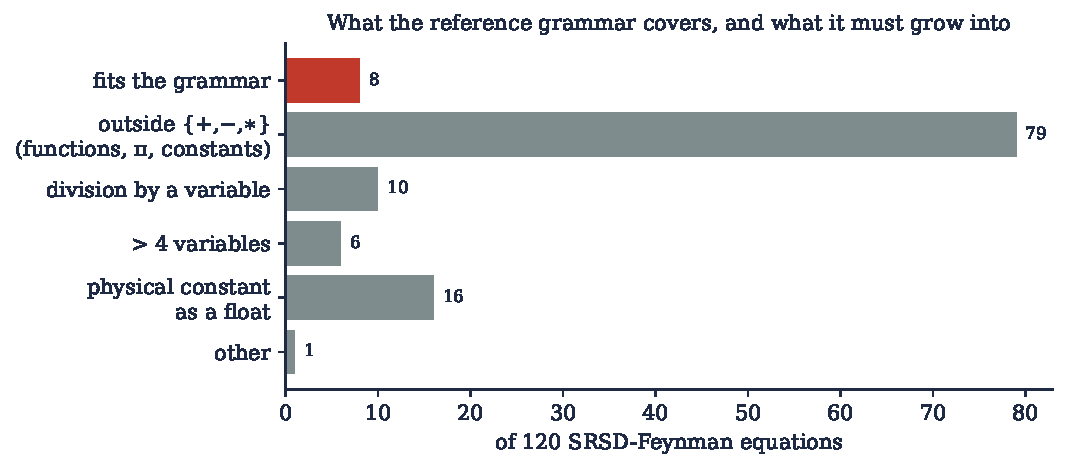
\includegraphics[width=0.78\textwidth]{fig_coverage}
\caption{Grammar coverage of SRSD-Feynman. Eight of 120 laws lie inside
$\{+,-,*\}$ with dyadic coefficients and at most four variables; the refusal
reasons are the roadmap for the grammar.}
\label{fig:coverage}
\end{figure}

8 of 120 laws fit ($6.7\%$). The five selected, smallest first and one per
algebraic shape, are I.12.1 ($F=\mu N$), I.39.10 ($E=\tfrac32 pV$), I.14.4
($U=\tfrac12 kx^2$), II.34.2 ($\mu = \tfrac12 qvr$) and II.37.1
($E=\mu B(1+\chi)$). Each was run with \texttt{kge solve} against random search
(the naive floor) and the restart hill-climber (the simple control) on the same
hundred seeds, twelve sample points and budget of $4{,}000$ evaluations, and
against the traditional method for a polynomial target --- exact regression over
the $35$ monomials of degree $\le 3$ in four variables, solved by Gaussian
elimination over the rationals --- in two regimes: on the same twelve points, and
on forty.

%% HF-RESULTS: generated by scripts/fill_paper_j_results.py
\begin{center}
\small
\begin{tabular}{llrrrrrll}
\toprule
 & & & \multicolumn{2}{c}{KGE} & climber & random & \multicolumn{2}{c}{exact regression} \\
law & form & size & rate & med.\ evals & rate & rate & 12 points & 40 points \\
\midrule
I.12.1 & $x0\,x1$ & 2 & 1.00 & 184 & 1.00 & 1.00 & ambiguous (null.\ 23) & exact \\
I.39.10 & $1.5\,x0\,x1$ & 3 & 0.51 & 1180 & 0.21 & 0.10 & ambiguous (null.\ 23) & exact \\
I.14.4 & $0.5\,x0\,x1^2$ & 4 & 0.07 & 525 & 0.27 & 0.20 & ambiguous (null.\ 23) & exact \\
II.34.2 & $x0\,x1\,x2/2$ & 4 & 0.22 & 1135 & 0.31 & 0.31 & ambiguous (null.\ 23) & exact \\
II.37.1 & $x0\,x2\,(x1 + 1)$ & 4 & 0.10 & 1102 & 0.16 & 0.15 & ambiguous (null.\ 23) & exact \\
\bottomrule
\end{tabular}
\end{center}

Across the five laws KGE solved 190 of 500 runs, the restart hill-climber 195 and random search 176. Every KGE solution was rendered to Lean and proved against the law by the kernel (\S\ref{sec:hubgate}). The traditional method is the honest foil: on the twelve points the search solves from, dense regression over 35 monomials is underdetermined for every law (nullity 23) and its particular solution does not reproduce the law on held-out points; given forty points it recovers each law exactly in about half a second with one or two nonzero terms. Which method wins depends on how much data there is: with few exact samples the search for a small expression recovers what a dense fit cannot pin down, and with enough samples linear algebra is faster and certain. KGE's distinctive contribution is not the recovery but what follows it --- a kernel proof that the recovered form equals the law. The population wins outright on 1 of the five laws (I.39.10) and is beaten by at least one of the two naive baselines on 3 (I.14.4, II.34.2, II.37.1). Every Hub law here has at most four leaves, which is the regime where the ladder already showed the population to be overhead (\S\ref{sec:climb}): for tiny targets, random search over small trees and a restart hill-climber are the better search layer, and the guideline in \S\ref{sec:guidelines} says so. The kernel gate is indifferent to which layer found the candidate.

\subsection{Kernel verdicts on the Hub solutions}\label{sec:hubgate}

%% HF-GATE: generated by scripts/fill_paper_j_results.py
Every distinct KGE solution (capped at eight per law) was rendered as a Lean definition with a theorem of equality to the law, and the batch for each law was compiled in one invocation with a deliberately wrong candidate (the law plus one) appended.

\begin{center}
\begin{tabular}{lrrrlrr}
\toprule
law & gated & proved & rejected & control rejected & invocations & wall clock \\
\midrule
I.12.1 & 8 & 8 & 0 & yes & 1 & 6.5\,s \\
I.39.10 & 8 & 8 & 0 & yes & 1 & 6.3\,s \\
I.14.4 & 7 & 7 & 0 & yes & 1 & 6.2\,s \\
II.34.2 & 8 & 8 & 0 & yes & 1 & 6.3\,s \\
II.37.1 & 8 & 8 & 0 & yes & 1 & 6.3\,s \\
\bottomrule
\end{tabular}
\end{center}

39 of 39 distinct solutions proved, in 5 invocations; the planted wrong candidate was rejected in every batch .

\section{Where KGE applies}\label{sec:applies}

\paragraph{Any synthesis with a formal acceptance criterion.} The architecture is
indifferent to the domain provided three things exist: an exact evaluator for
candidates, a renderable specification, and a kernel that can decide equality.
The search layer can be replaced wholesale; the guarantee is in the gate.
Concretely: rewriting rules in a compiler whose equivalence must be certified;
algebraic simplifications in a computer-algebra pipeline; closed-form identities
conjectured from data and then proved rather than tested.

\paragraph{Lean-gated numerical kernels.} The motivating case: evolving a
candidate kernel (an integrator step, a stencil, an update rule, a
finite-difference coefficient set) that must be \emph{proved} equal to a
specification before it enters a simulation. KGE finds candidates by exact
fitness, removes most wrong ones at zero kernel cost, and proves the survivors in
batches. The Verlet position update is the worked example; the same shape covers
symplectic integrators, conservation-law discretisations and any update rule
expressible over the grammar.

\paragraph{Inert-locus analysis of evolved programs.} Inert loci are identified
exactly, not statistically, from the dosage coefficients. Evolved programs are
notorious for bloat; KGE measures it as a fraction of loci that cannot reach the
phenotype and can prune it with no change in behaviour. The same analysis gives
an exact sensitivity map of any program over the grammar: which inputs reach the
output, and with what coefficient, at every point.

\paragraph{eXpensive verification, batched.} The one-invocation gate is
independent of KGE: any pipeline that verifies candidates in Lean --- an
LLM-driven prover loop, a conjecture miner, a refactoring assistant --- can read
the per-declaration report and verify a batch at the price of one, at any
failure rate, with every culprit named.

\paragraph{Rediscovery of laws from exact data.} Where a physical law is
polynomial in its variables with small rational coefficients (\S\ref{sec:hub}
measures how often that holds), KGE recovers it from a dozen exact samples and
proves the recovered form, where dense regression on the same samples is
underdetermined. The complement --- laws with constants, roots and transcendental
functions --- is the grammar's roadmap, not its claim.

\section{Guidelines: where and how to use KGE}\label{sec:guidelines}

\paragraph{When to reach for it.} Use KGE when a candidate's acceptance must be
\emph{formal} rather than empirical, when an exact evaluator exists for the
candidate representation, and when the specification can be rendered as a Lean
definition. If any of the three is missing, the kernel gate is the piece to keep
and the search layer the piece to swap.

\paragraph{eXact first.} Keep every quantity the search sees exact. The
checkpoint's soundness and the dosage identities both rest on exact arithmetic;
a floating-point fitness would turn refutations into guesses.

\paragraph{Arbiter before operator.} Build and test the kernel gate with a
planted wrong candidate in every batch \emph{before} tuning any variation
operator. A gate that cannot reject is worse than none, and no operator result
means anything until the gate is shown to refuse.

\paragraph{Verify against the simplest control.} Run the restart hill-climber on
the same seeds, points and budget before claiming anything for the population,
and report McNemar on the discordant pairs. On easy targets the climber wins
(\S\ref{sec:climb}); design the population in because the hard rungs need it,
not because the method is called genetic.

\paragraph{Calibrate difficulty on a pooled band.} Choose benchmark targets by a
pooled success-rate band fixed in advance, so that neither trivial nor
impossible targets masquerade as a comparison, and never by the rung that
flatters a method.

\paragraph{Report both costs.} Fitness evaluations and total tree-point
evaluations, always. An operator that probes the genome spends compute the
budget does not see; a win in one currency and a loss in the other is a loss.

\paragraph{Replay, do not inspect.} When two implementations disagree, replay
one on the other's exact sample points. A solve rate that moves with the points
is a property of the landscape instance, not a bug.

\paragraph{Grow the grammar deliberately.} Every refusal in \S\ref{sec:hub} is a
feature request with a count attached: division by a variable, transcendental
functions, physical constants. Add them with their dosage rule proved, as the
three operators here are, or not at all.

\section{Significance}\label{sec:significance}

\paragraph{For science.} The step that scientific computing most needs and least
has is a mechanical bridge from a candidate formula to a certified one. KGE
makes that bridge the \emph{default} output of a search: what comes out is not a
formula that fits, but a formula with a kernel-checked proof that it equals the
specification on the whole domain. For laws inside the grammar, that is
rediscovery with a proof attached, from a dozen exact samples.

\paragraph{For verified software.} Numerical kernels in simulators, control
systems and scientific libraries are routinely hand-derived and empirically
tested. A pipeline that evolves them and refuses to accept without a proof moves
the guarantee from the test suite to the kernel, and does so at one invocation
per batch of candidates.

\paragraph{For the collaboration between people and machines.} The division of
labour KGE enforces --- the search may be heuristic, biological, even wrong,
because the kernel decides --- is a model for working with AI systems in general:
let the generator be creative and the arbiter be formal, and never let the
generator grade itself. Every control in this paper exists because that
principle was applied to our own work as well as to the machine's.

\section{Limitations}

\begin{itemize}
\item \textbf{Scope of the reference implementation.} One closed grammar
$\{+,-,*\}$, four variables, three constants, one specification family. The
architecture is general; the measurements are not.
\item \textbf{Scaling.} Solve rates fall steeply above targets of about nine
nodes, and the full Verlet target (size 17) is not solved within $4{,}000$
evaluations. The cliff is not explained by the geometry of the basin around the
solution (measured) and is not relieved by recombination: eight variation
operators including homologous, contribution-preserving and semantically
back-propagated variants were tested against mutation under pre-registered bars
and none improved on it, which is why KGE is mutation-driven. The evidence
points at how hard the basin is to find in a growing space, not at how it is
shaped. (Companion measurements: Paper~I, DOI 10.5281/zenodo.23622868.)
\item \textbf{The checkpoint is one-sided by design.} A candidate can be tuned
to agree at the sample points and still be wrong; it survives the checkpoint and
costs a kernel invocation before being rejected. This is a cost, never a
soundness risk, and is reduced by drawing sample points per generation.
\item \textbf{Dosage is instrumentation.} As a guide for variation operators it
did not improve search outcomes in our tests; its value here is exact analysis
and exact pruning, not steering.
\item \textbf{Fixed per-invocation cost.} About $97\%$ of a Lean invocation is
fixed overhead on this host. Batching amortises it; a persistent kernel process
would remove it and was not built.
\end{itemize}

\section{Future research}

\begin{enumerate}
\item \textbf{Keep exploiting the affine structure.} Because the output is
affine in every locus, constant loci could be solved by exact linear algebra
rather than searched; a genome of structural operators with coefficients fitted
exactly would turn part of the search into a solve --- and
\S\ref{sec:hub} shows exactly where dense regression needs more data than the
search does, so the hybrid has a measured motivation.
\item \textbf{Adaptive checkpoints.} Sample points redrawn each generation defeat
evaders at no proof cost and bound how long a wrong survivor can persist.
\item \textbf{Lean kernel, persistent.} Removing the fixed per-invocation cost
would make the gate nearly free per candidate and change what batch sizes are
optimal.
\item \textbf{Grammar growth with proofs.} Division, powers and the common
transcendental functions, each added with its dosage rule proved in
\texttt{AlixKalSpec.lean}; the SRSD-Feynman refusals in Fig.~\ref{fig:coverage}
rank them by how many laws each would unlock.
\item \textbf{Representations with higher solution density at scale.} The cliff
is about finding basins in a growing space; semantic deduplication of the
population is the natural lever once the grammar is richer.
\item \textbf{Contribution-preserving transfer, properly powered.} Rescaling a
transplanted subtree so its dosage-weighted contribution is preserved exactly
showed a positive signal against its matched control ($p=0.031$, not surviving
correction for five comparisons) and merits a dedicated study.
\item \textbf{Application to the project's Python-genome kernel path.} The
AlphaEvolve-style path evolves Python kernels; KGE's checkpoint and gate apply
unchanged once a Lean specification exists for the kernel being evolved.
\end{enumerate}

\section{Reproduction}

The Rust crate, its tests, the ladder runs and the gate results are deposited
alongside this paper, together with the Python prototype in which the identities
were first verified and the verifier whose per-declaration report makes the
one-invocation gate possible. Every number above is produced by a committed
script or test and is checked against its artefact before deposit.

\end{document}
